
\section{Implementation and Evaluation}
\label{sec:eval}

We have implemented a tool, \app, and evaluated it based on real-world configuration files taken from Github.
\app is written in Haskell and is available open source at \textit{url redacted for anonymity}.
Thanks to the Haskell's powerful type system, the implementation can easily be extended with new rule classes or applied to different configuration languages with minimal change to the rest of the code base.
A user only needs to provide the functions for the rule interface (a typeclass in Haskell) to 1) learn relations from a single file 2) merge two sets of rules and 3) check a file given some set of rules.

\subsection{Evaluation}

To evaluate our \app prototype, we require a separate training set and test set. 
For our training set, \trainingSet, we use a preexisting set of 256 
industrial MySQL configuration files collected in previous configuration 
analysis work~\cite{configdataset}.
This is an unlabeled training set, though most of the files have some errors.
For our test set, we collected 1000 MySQL configuration files 
from Github, and filtered the incorrectly formatted files out for a final 
total of 973 files.
In our evaluation, we focus on MySQL for comparability of results, but \app can handle any configuration language (that can be parsed to the intermediate representation from Sec.~\ref{sec:trans}).

We report the number of rules learned from the training set and the number of errors detected in the test set in Table~\ref{table:learning}.
One interesting note is that without probabilistic types we learned 327 fine grained rules and detected 1367 errors.
By introducing probabilistic types, we remove 114 incorrect rules and thereby remove 1023 false positives.
We are guaranteed these are all false positives since there cannot be a correct rule of relating the types $size*size$ and $size$ because of the semantic interpretation of the $size$ units.

We also provide the support and confidence thresholds, $t_s, t_c$, used in this evaluation.
These number can be adjusted by the user as a slider to control the level of assurance that their file is correct.
Since these settings depend on both the user preference and training set quality, we simply choose values for which \app reports reasonably sized output.

We record the histogram of errors across the test set in Figure~\ref{fig:histo}.
This is intuitively an expected result from randomly sampling Github - most repositories will have few errors, with an increasingly small number of repositories having many errors.

\begin{figure}[h]
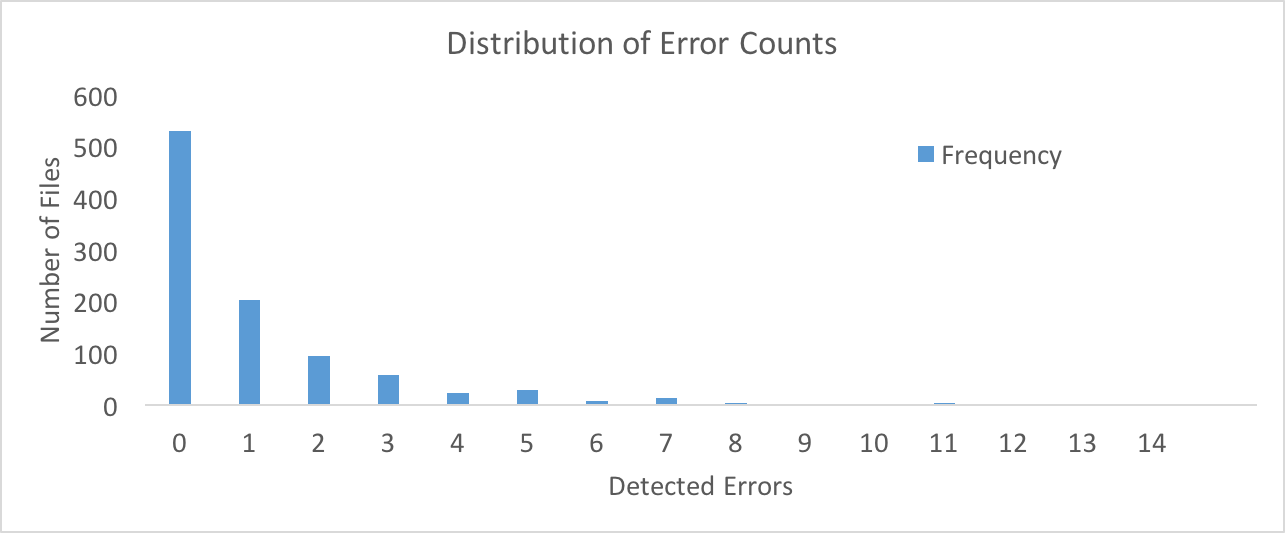
\includegraphics[width=\textwidth]{figs/histogram.png}
\caption{Histogram of errors - 14 errors were detected in 1 file}
\label{fig:histo}
\end{figure}

\begin{table}[h]
\centering
\caption{Results of \app}
\label{table:learning}
\setlength{\tabcolsep}{0.5em}
\begin{tabular}{|c|c|c|c|c|}
\hline
{\bf Class of Error } & {\bf \# Rules Learned} & {\bf \# Errors Detected} & {\bf Support} & {\bf Confidence}\\ 
\hline
\hline
Order        & 13  & 62   & 6 \%  & 94 \% \\ 
Missing      & 53  & 55   & 2 \%  & 71\% \\ 
Type         & 92  & 389  & 12 \% & 70\%  \\ 
Fine-Grain   & 213 & 324  & 24 \% & 91\%  \\ 
Coarse-Grain & 97  & 237  & 10 \% & 96\% \\ 
\hline 
\end{tabular}
\end{table}

The errors reported may have varying impacts on the system, ranging from failing to start, runtime crash, or performance degradation.
However, since \app is a probabilistic system, it is also possible that some errors are false positives, a violation of the rule has no effect on the system.
Note that in contrast to program verification, we do not have an oracle for determining if a reported error is a true error or a false positive.
While we can run a program to determine the effect a specification has on the success of compiling/running the program, no such test exists for configuration files.
Because configurations are dependent on the rest of the system (\ie, the available hardware, the network speed, and the usage patterns), we cannot simulate the all conditions to determine if a reported error will cause system failure.
As evidenced by Example~\ref{ex:fine}, some misconfigurations will only cause greater than expected performance degradation, and only under particular traffic loads.
In light of this, the definition of a true error is necessarily imprecise.

Although we cannot identify false positives, we can identify true positives by examining online forums, like StackOverflow.
On these forums we find reports that particular configuration settings have caused problems on real-world systems.
Furthermore, any error for which we can find evidence online is likely to be more problematic than errors that do not have an online record, 
  using the reasoning that this error has caused enough problems for people to seek help online.
In this case, we would like \app to sort the errors by their importance or potential severity.
To achieve this sorting we use the rule graph analysis metric described in Sec.~\ref{sec:ruleorder}.

To estimate the impact of this metric, we track the rank of known true positives with, and without, the augmented rule ordering in Table~\ref{table-casestudy}.
For this table, we picked the known true positive rules, listed in the Errors column, and pick configuration files in the test set that have these errors.
We picked 3 files for each true positive by choosing the files with the highest number of total reported errors in order to clearly observe the effects of our optimizations.
Although this gives a more clear picture of the effect of our optimizations, it results in a slightly inflated false positive rate.

We test the following conditions; just rule graph analysis (RG) to sort the errors, just probabilistic types to filter the rules (PT), and both optimizations at the same time (RG $\land$ PT).
For each entry we list X/Y, where X is the rank of the known true positive, and Y is the total number of errors found in that file.


\newcommand{\tablewidth}{6cm}
\definecolor{Gray}{gray}{0.80}
\newcolumntype{g}{>{\columncolor{Gray}}c}


\begin{table*}[tbp]
\centering
\caption{Sampled misconfiguration files for error detection evaluation.}
\label{table-casestudy}
\setlength{\tabcolsep}{0.5em}
\begin{footnotesize}
\begin{tabular}{|c|c|c|g|g|c|}
\hline
{\bf Errors} & {\bf URLs} & {\bf None} & {\bf PA} & {\bf PT} & {\bf PT$\land$ PA}\\ 
\hline
\hline
\multirow{3}{*}{\parbox{\tablewidth} {\scriptsize ORDERING ERROR: Expected ``innodb\_data\_home\_dir'' BEFORE ``innodb\_data\_file\_path''} }
& url & 12/12 & 3/12 & 5/5 & 3/5 \\
& url & 11/11 & 2/11 & 3/3 & 3/3 \\ 
& url & 9/9   & 3/9  & 4/4 & 3/4 \\ 
\hline

\multirow{3}{*}{\parbox{\tablewidth} {\scriptsize MISSING ERROR: Expected ``key\_buffer'' WITH [isamchk]} }
& url & 6/10 & 2/10 & 2/4 & 2/4 \\ 
& url & 2/3 & 3/3 & 2/3 & 3/3 \\
& url & 2/3 & 3/3 & 2/2 & 3/3 \\  
\hline

\multirow{3}{*}{\parbox{\tablewidth} {\scriptsize TYPE ERROR: Expected an integer for “slow\_query\_log”}}
& url & 32/34 & 1/34 & 5/7   & 1/7 \\ 
& url & 9/20  & 2/20 & 10/11 & 2/11 \\  
& url & 9/19  & 2/19 & 10/11 & 2/11 \\
\hline

\multirow{3}{*}{\parbox{\tablewidth} {\scriptsize FINE GRAINED ERROR: Expected \\ ``max\_connections'' * ``sort\_buffer\_size'' $\geq$ ``key\_buffer\_size''}}
& url & 30/34 & 18/24 & 6/7 & 3/7 \\ 
& url & 23/25 & 9/25  & 8/9 & 3/9 \\  
& url & 20/23 & 14/23 & 6/7 & 5/7 \\
\hline

\multirow{3}{*}{\parbox{\tablewidth} {\scriptsize INTEGER CORRELATION ERROR: Expected ``max\_allowed\_packet'' $<$ ``innodb\_buffer\_pool\_size''} }
& url & 29/32 & 8/32 & 11/14 & 4/14 \\ 
& url & 22/23 & 2/23 & 9/10  & 2/10 \\  
& url & 10/12 & 4/12 & 4/4   & 2/4 \\
\hline

\end{tabular}
\end{footnotesize}
\end{table*}




\subsection{False Positive Rate}

Because \app detects complex and subtle misconfigurations that, for example, may cause performance degradation in a high traffic load, false positives are system and use-case dependent and therefore ill-defined.
However, we report an estimation of the false positive rate for comparison to other tools.
To estimate a false positive rate, we asked two industry experts, one from MongoDB and one from Microsoft, to independently classify all errors from Table~\ref{table-casestudy}.
For each unique error reported in Table~\ref{table-casestudy} (a total of 70 unique errors), the expert was asked to classify the error as: definitely false positive, potential true positive, or definitely true positive. 
The MongoDB expert rated 13/70 errors as definitely false positives. 
The Microsoft expert rated 8/70 errors as definitely false positives. 
The similarity between experts is suggestive that these are approximately correct classifications.

The resulting false positive rate is then estimated to be 11\%-18\%.
This is in the range of existing work, for example in the EnCore tool, which had a false positive rate of 13\%,21\%,32\% for MySQL, Apache, and PHP respectively~\cite{encore}.
We note again that as opposed to a tool like EnCore, which is used mainly to detect initialization errors, thanks to the complex relations that can be learned, \app also learns misconfigurations causing runtime performance degradation.
This means \app generates a larger rule set, and false positives cannot be garunteed, i.e. there may be some environment conditions that will cause a ``false'' positive to become a true positive.

In contrast, a true positive can be confirmed as such based on evidence of unwanted system behvaior.
The errors listed in Table~\ref{table-casestudy} are confirmed true positives, evidenced by posts on help forums.
\app detected and reports these errors in the 15 code repositories listed in the URL column of Table~\ref{table-casestudy}. 
These are real-world configuration files that contain errors that may be unknown to the maintainers of the repositories.
%The errors were not submitted as patches to the repository owners, since it is possible the owner of the repository has a user case for this configuration file that will not trigger the unwanted behavior.

\subsection{Runtime Performance}
We also evaluate the speed of \app.
Generally, once a set of rules has been learned, it is not necessary to rerun the learner.
However, we have only used \app to build rules for MySQL, but any configuration language can be analyzed with \app given a training set, which requires rerunning the learner.
Additionally, in an industrial setting, the available training set may be much larger than ours, so is important that the learning process scales.
We see in Table~\ref{table:training} that \app scales roughly linearly.

We compare \app to prior work in configuration verification, ConfigC~\cite{santolucitoCAV}.
ConfigC scales exponentially because the learning algorithm assumes a completely correct training set, and learns every derivable relation.
With \app, we instead only process rules that meet the required support and confidence, reducing the cost of resolving to a consistent set of rules. 
The times reported in Table~\ref{table:training} were run on four cores of a Kaby Lake Intel Core i7-7500U CPU @ 2.70GHz on 16GB RAM and Fedora 25.

\begin{table}[h!]
\centering
\caption{Time for training over various training set sizes}
\label{table:training}
\setlength{\tabcolsep}{1em}
\begin{tabular}{|c|c|c|}
\hline
{\bf \# of Files for Training} & {\bf ConfigC (sec)} & {\bf \app (sec)}\\ 
\hline
\hline
0    & 0.051    & 0.051  \\ \hline
50   & 1.815    & 1.638  \\ \hline
100  & 13.331   & 4.119  \\ \hline
150  & 95.547   & 10.232  \\ \hline
200  & 192.882  & 12.271  \\ \hline
256  & 766.904  & 15.627  \\ 
\hline
\end{tabular}
\end{table}

